% generated by check.py from the computed solutions; do not edit
\newcommand{\MthreeSola}{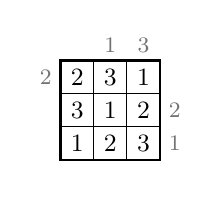
\begin{tikzpicture}[x=0.42cm,y=0.42cm]
\draw[line width=0.4pt] (1,0) -- (1,3);
\draw[line width=0.4pt] (0,1) -- (3,1);
\draw[line width=0.4pt] (2,0) -- (2,3);
\draw[line width=0.4pt] (0,2) -- (3,2);
\draw[line width=1pt] (0,0) rectangle (3,3);
\node at (0.5,2.5) {\small 2};
\node at (1.5,2.5) {\small 3};
\node at (2.5,2.5) {\small 1};
\node at (0.5,1.5) {\small 3};
\node at (1.5,1.5) {\small 1};
\node at (2.5,1.5) {\small 2};
\node at (0.5,0.5) {\small 1};
\node at (1.5,0.5) {\small 2};
\node at (2.5,0.5) {\small 3};
\node[text=black!55] at (1.5,3.45) {\footnotesize 1};
\node[text=black!55] at (2.5,3.45) {\footnotesize 3};
\node[text=black!55] at (-0.45,2.5) {\footnotesize 2};
\node[text=black!55] at (3.45,1.5) {\footnotesize 2};
\node[text=black!55] at (3.45,0.5) {\footnotesize 1};
\path (-1,-1) rectangle (4,4);
\end{tikzpicture}}
\newcommand{\MthreeSolb}{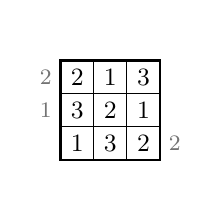
\begin{tikzpicture}[x=0.42cm,y=0.42cm]
\draw[line width=0.4pt] (1,0) -- (1,3);
\draw[line width=0.4pt] (0,1) -- (3,1);
\draw[line width=0.4pt] (2,0) -- (2,3);
\draw[line width=0.4pt] (0,2) -- (3,2);
\draw[line width=1pt] (0,0) rectangle (3,3);
\node at (0.5,2.5) {\small 2};
\node at (1.5,2.5) {\small 1};
\node at (2.5,2.5) {\small 3};
\node at (0.5,1.5) {\small 3};
\node at (1.5,1.5) {\small 2};
\node at (2.5,1.5) {\small 1};
\node at (0.5,0.5) {\small 1};
\node at (1.5,0.5) {\small 3};
\node at (2.5,0.5) {\small 2};
\node[text=black!55] at (-0.45,2.5) {\footnotesize 2};
\node[text=black!55] at (-0.45,1.5) {\footnotesize 1};
\node[text=black!55] at (3.45,0.5) {\footnotesize 2};
\path (-1,-1) rectangle (4,4);
\end{tikzpicture}}
\newcommand{\MthreeSold}{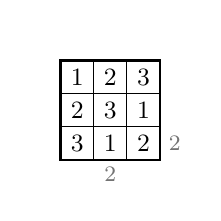
\begin{tikzpicture}[x=0.42cm,y=0.42cm]
\draw[line width=0.4pt] (1,0) -- (1,3);
\draw[line width=0.4pt] (0,1) -- (3,1);
\draw[line width=0.4pt] (2,0) -- (2,3);
\draw[line width=0.4pt] (0,2) -- (3,2);
\draw[line width=1pt] (0,0) rectangle (3,3);
\node at (0.5,2.5) {\small 1};
\node at (1.5,2.5) {\small 2};
\node at (2.5,2.5) {\small 3};
\node at (0.5,1.5) {\small 2};
\node at (1.5,1.5) {\small 3};
\node at (2.5,1.5) {\small 1};
\node at (0.5,0.5) {\small 3};
\node at (1.5,0.5) {\small 1};
\node at (2.5,0.5) {\small 2};
\node[text=black!55] at (3.45,0.5) {\footnotesize 2};
\node[text=black!55] at (1.5,-0.45) {\footnotesize 2};
\path (-1,-1) rectangle (4,4);
\end{tikzpicture}}
\newcommand{\MfourSola}{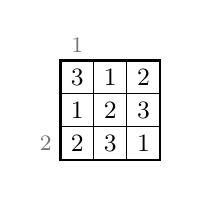
\begin{tikzpicture}[x=0.42cm,y=0.42cm]
\draw[line width=0.4pt] (1,0) -- (1,3);
\draw[line width=0.4pt] (0,1) -- (3,1);
\draw[line width=0.4pt] (2,0) -- (2,3);
\draw[line width=0.4pt] (0,2) -- (3,2);
\draw[line width=1pt] (0,0) rectangle (3,3);
\node at (0.5,2.5) {\small 3};
\node at (1.5,2.5) {\small 1};
\node at (2.5,2.5) {\small 2};
\node at (0.5,1.5) {\small 1};
\node at (1.5,1.5) {\small 2};
\node at (2.5,1.5) {\small 3};
\node at (0.5,0.5) {\small 2};
\node at (1.5,0.5) {\small 3};
\node at (2.5,0.5) {\small 1};
\node[text=black!55] at (0.5,3.45) {\footnotesize 1};
\node[text=black!55] at (-0.45,0.5) {\footnotesize 2};
\path (-1,-1) rectangle (4,4);
\end{tikzpicture}}
\newcommand{\MfourSolb}{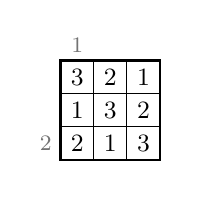
\begin{tikzpicture}[x=0.42cm,y=0.42cm]
\draw[line width=0.4pt] (1,0) -- (1,3);
\draw[line width=0.4pt] (0,1) -- (3,1);
\draw[line width=0.4pt] (2,0) -- (2,3);
\draw[line width=0.4pt] (0,2) -- (3,2);
\draw[line width=1pt] (0,0) rectangle (3,3);
\node at (0.5,2.5) {\small 3};
\node at (1.5,2.5) {\small 2};
\node at (2.5,2.5) {\small 1};
\node at (0.5,1.5) {\small 1};
\node at (1.5,1.5) {\small 3};
\node at (2.5,1.5) {\small 2};
\node at (0.5,0.5) {\small 2};
\node at (1.5,0.5) {\small 1};
\node at (2.5,0.5) {\small 3};
\node[text=black!55] at (0.5,3.45) {\footnotesize 1};
\node[text=black!55] at (-0.45,0.5) {\footnotesize 2};
\path (-1,-1) rectangle (4,4);
\end{tikzpicture}}
\newcommand{\MfourSolc}{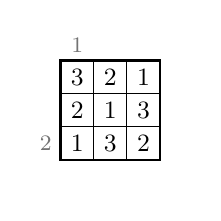
\begin{tikzpicture}[x=0.42cm,y=0.42cm]
\draw[line width=0.4pt] (1,0) -- (1,3);
\draw[line width=0.4pt] (0,1) -- (3,1);
\draw[line width=0.4pt] (2,0) -- (2,3);
\draw[line width=0.4pt] (0,2) -- (3,2);
\draw[line width=1pt] (0,0) rectangle (3,3);
\node at (0.5,2.5) {\small 3};
\node at (1.5,2.5) {\small 2};
\node at (2.5,2.5) {\small 1};
\node at (0.5,1.5) {\small 2};
\node at (1.5,1.5) {\small 1};
\node at (2.5,1.5) {\small 3};
\node at (0.5,0.5) {\small 1};
\node at (1.5,0.5) {\small 3};
\node at (2.5,0.5) {\small 2};
\node[text=black!55] at (0.5,3.45) {\footnotesize 1};
\node[text=black!55] at (-0.45,0.5) {\footnotesize 2};
\path (-1,-1) rectangle (4,4);
\end{tikzpicture}}
\newcommand{\UthreeSola}{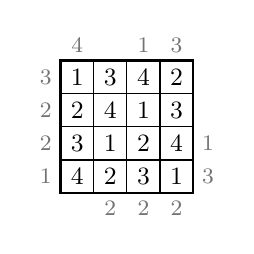
\begin{tikzpicture}[x=0.42cm,y=0.42cm]
\draw[line width=0.4pt] (1,0) -- (1,4);
\draw[line width=0.4pt] (0,1) -- (4,1);
\draw[line width=0.4pt] (2,0) -- (2,4);
\draw[line width=0.4pt] (0,2) -- (4,2);
\draw[line width=0.4pt] (3,0) -- (3,4);
\draw[line width=0.4pt] (0,3) -- (4,3);
\draw[line width=1pt] (0,0) rectangle (4,4);
\node at (0.5,3.5) {\small 1};
\node at (1.5,3.5) {\small 3};
\node at (2.5,3.5) {\small 4};
\node at (3.5,3.5) {\small 2};
\node at (0.5,2.5) {\small 2};
\node at (1.5,2.5) {\small 4};
\node at (2.5,2.5) {\small 1};
\node at (3.5,2.5) {\small 3};
\node at (0.5,1.5) {\small 3};
\node at (1.5,1.5) {\small 1};
\node at (2.5,1.5) {\small 2};
\node at (3.5,1.5) {\small 4};
\node at (0.5,0.5) {\small 4};
\node at (1.5,0.5) {\small 2};
\node at (2.5,0.5) {\small 3};
\node at (3.5,0.5) {\small 1};
\node[text=black!55] at (0.5,4.45) {\footnotesize 4};
\node[text=black!55] at (2.5,4.45) {\footnotesize 1};
\node[text=black!55] at (3.5,4.45) {\footnotesize 3};
\node[text=black!55] at (-0.45,3.5) {\footnotesize 3};
\node[text=black!55] at (-0.45,2.5) {\footnotesize 2};
\node[text=black!55] at (-0.45,1.5) {\footnotesize 2};
\node[text=black!55] at (-0.45,0.5) {\footnotesize 1};
\node[text=black!55] at (4.45,1.5) {\footnotesize 1};
\node[text=black!55] at (4.45,0.5) {\footnotesize 3};
\node[text=black!55] at (1.5,-0.45) {\footnotesize 2};
\node[text=black!55] at (2.5,-0.45) {\footnotesize 2};
\node[text=black!55] at (3.5,-0.45) {\footnotesize 2};
\path (-1,-1) rectangle (5,5);
\end{tikzpicture}}
\newcommand{\UthreeSolb}{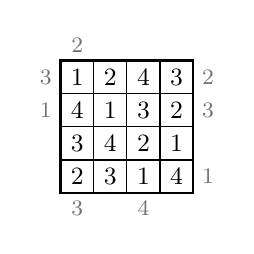
\begin{tikzpicture}[x=0.42cm,y=0.42cm]
\draw[line width=0.4pt] (1,0) -- (1,4);
\draw[line width=0.4pt] (0,1) -- (4,1);
\draw[line width=0.4pt] (2,0) -- (2,4);
\draw[line width=0.4pt] (0,2) -- (4,2);
\draw[line width=0.4pt] (3,0) -- (3,4);
\draw[line width=0.4pt] (0,3) -- (4,3);
\draw[line width=1pt] (0,0) rectangle (4,4);
\node at (0.5,3.5) {\small 1};
\node at (1.5,3.5) {\small 2};
\node at (2.5,3.5) {\small 4};
\node at (3.5,3.5) {\small 3};
\node at (0.5,2.5) {\small 4};
\node at (1.5,2.5) {\small 1};
\node at (2.5,2.5) {\small 3};
\node at (3.5,2.5) {\small 2};
\node at (0.5,1.5) {\small 3};
\node at (1.5,1.5) {\small 4};
\node at (2.5,1.5) {\small 2};
\node at (3.5,1.5) {\small 1};
\node at (0.5,0.5) {\small 2};
\node at (1.5,0.5) {\small 3};
\node at (2.5,0.5) {\small 1};
\node at (3.5,0.5) {\small 4};
\node[text=black!55] at (0.5,4.45) {\footnotesize 2};
\node[text=black!55] at (-0.45,3.5) {\footnotesize 3};
\node[text=black!55] at (-0.45,2.5) {\footnotesize 1};
\node[text=black!55] at (4.45,3.5) {\footnotesize 2};
\node[text=black!55] at (4.45,2.5) {\footnotesize 3};
\node[text=black!55] at (4.45,0.5) {\footnotesize 1};
\node[text=black!55] at (0.5,-0.45) {\footnotesize 3};
\node[text=black!55] at (2.5,-0.45) {\footnotesize 4};
\path (-1,-1) rectangle (5,5);
\end{tikzpicture}}
\newcommand{\UthreeSolc}{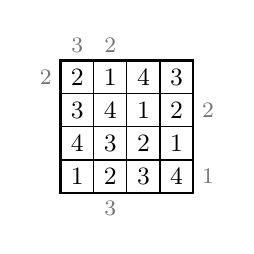
\begin{tikzpicture}[x=0.42cm,y=0.42cm]
\draw[line width=0.4pt] (1,0) -- (1,4);
\draw[line width=0.4pt] (0,1) -- (4,1);
\draw[line width=0.4pt] (2,0) -- (2,4);
\draw[line width=0.4pt] (0,2) -- (4,2);
\draw[line width=0.4pt] (3,0) -- (3,4);
\draw[line width=0.4pt] (0,3) -- (4,3);
\draw[line width=1pt] (0,0) rectangle (4,4);
\node at (0.5,3.5) {\small 2};
\node at (1.5,3.5) {\small 1};
\node at (2.5,3.5) {\small 4};
\node at (3.5,3.5) {\small 3};
\node at (0.5,2.5) {\small 3};
\node at (1.5,2.5) {\small 4};
\node at (2.5,2.5) {\small 1};
\node at (3.5,2.5) {\small 2};
\node at (0.5,1.5) {\small 4};
\node at (1.5,1.5) {\small 3};
\node at (2.5,1.5) {\small 2};
\node at (3.5,1.5) {\small 1};
\node at (0.5,0.5) {\small 1};
\node at (1.5,0.5) {\small 2};
\node at (2.5,0.5) {\small 3};
\node at (3.5,0.5) {\small 4};
\node[text=black!55] at (0.5,4.45) {\footnotesize 3};
\node[text=black!55] at (1.5,4.45) {\footnotesize 2};
\node[text=black!55] at (-0.45,3.5) {\footnotesize 2};
\node[text=black!55] at (4.45,2.5) {\footnotesize 2};
\node[text=black!55] at (4.45,0.5) {\footnotesize 1};
\node[text=black!55] at (1.5,-0.45) {\footnotesize 3};
\path (-1,-1) rectangle (5,5);
\end{tikzpicture}}
\newcommand{\UthreeSold}{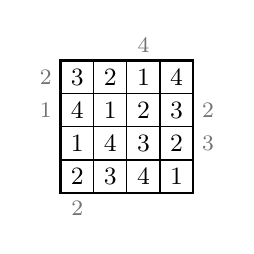
\begin{tikzpicture}[x=0.42cm,y=0.42cm]
\draw[line width=0.4pt] (1,0) -- (1,4);
\draw[line width=0.4pt] (0,1) -- (4,1);
\draw[line width=0.4pt] (2,0) -- (2,4);
\draw[line width=0.4pt] (0,2) -- (4,2);
\draw[line width=0.4pt] (3,0) -- (3,4);
\draw[line width=0.4pt] (0,3) -- (4,3);
\draw[line width=1pt] (0,0) rectangle (4,4);
\node at (0.5,3.5) {\small 3};
\node at (1.5,3.5) {\small 2};
\node at (2.5,3.5) {\small 1};
\node at (3.5,3.5) {\small 4};
\node at (0.5,2.5) {\small 4};
\node at (1.5,2.5) {\small 1};
\node at (2.5,2.5) {\small 2};
\node at (3.5,2.5) {\small 3};
\node at (0.5,1.5) {\small 1};
\node at (1.5,1.5) {\small 4};
\node at (2.5,1.5) {\small 3};
\node at (3.5,1.5) {\small 2};
\node at (0.5,0.5) {\small 2};
\node at (1.5,0.5) {\small 3};
\node at (2.5,0.5) {\small 4};
\node at (3.5,0.5) {\small 1};
\node[text=black!55] at (2.5,4.45) {\footnotesize 4};
\node[text=black!55] at (-0.45,3.5) {\footnotesize 2};
\node[text=black!55] at (-0.45,2.5) {\footnotesize 1};
\node[text=black!55] at (4.45,2.5) {\footnotesize 2};
\node[text=black!55] at (4.45,1.5) {\footnotesize 3};
\node[text=black!55] at (0.5,-0.45) {\footnotesize 2};
\path (-1,-1) rectangle (5,5);
\end{tikzpicture}}
\newcommand{\UthreeSole}{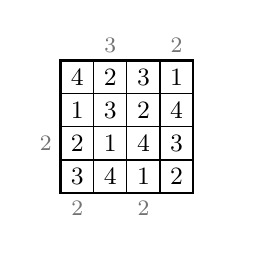
\begin{tikzpicture}[x=0.42cm,y=0.42cm]
\draw[line width=0.4pt] (1,0) -- (1,4);
\draw[line width=0.4pt] (0,1) -- (4,1);
\draw[line width=0.4pt] (2,0) -- (2,4);
\draw[line width=0.4pt] (0,2) -- (4,2);
\draw[line width=0.4pt] (3,0) -- (3,4);
\draw[line width=0.4pt] (0,3) -- (4,3);
\draw[line width=1pt] (0,0) rectangle (4,4);
\node at (0.5,3.5) {\small 4};
\node at (1.5,3.5) {\small 2};
\node at (2.5,3.5) {\small 3};
\node at (3.5,3.5) {\small 1};
\node at (0.5,2.5) {\small 1};
\node at (1.5,2.5) {\small 3};
\node at (2.5,2.5) {\small 2};
\node at (3.5,2.5) {\small 4};
\node at (0.5,1.5) {\small 2};
\node at (1.5,1.5) {\small 1};
\node at (2.5,1.5) {\small 4};
\node at (3.5,1.5) {\small 3};
\node at (0.5,0.5) {\small 3};
\node at (1.5,0.5) {\small 4};
\node at (2.5,0.5) {\small 1};
\node at (3.5,0.5) {\small 2};
\node[text=black!55] at (1.5,4.45) {\footnotesize 3};
\node[text=black!55] at (3.5,4.45) {\footnotesize 2};
\node[text=black!55] at (-0.45,1.5) {\footnotesize 2};
\node[text=black!55] at (0.5,-0.45) {\footnotesize 2};
\node[text=black!55] at (2.5,-0.45) {\footnotesize 2};
\path (-1,-1) rectangle (5,5);
\end{tikzpicture}}
\newcommand{\UthreeSolf}{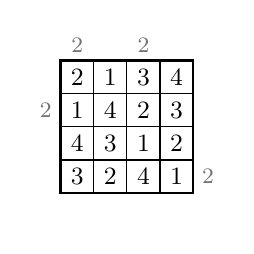
\begin{tikzpicture}[x=0.42cm,y=0.42cm]
\draw[line width=0.4pt] (1,0) -- (1,4);
\draw[line width=0.4pt] (0,1) -- (4,1);
\draw[line width=0.4pt] (2,0) -- (2,4);
\draw[line width=0.4pt] (0,2) -- (4,2);
\draw[line width=0.4pt] (3,0) -- (3,4);
\draw[line width=0.4pt] (0,3) -- (4,3);
\draw[line width=1pt] (0,0) rectangle (4,4);
\node at (0.5,3.5) {\small 2};
\node at (1.5,3.5) {\small 1};
\node at (2.5,3.5) {\small 3};
\node at (3.5,3.5) {\small 4};
\node at (0.5,2.5) {\small 1};
\node at (1.5,2.5) {\small 4};
\node at (2.5,2.5) {\small 2};
\node at (3.5,2.5) {\small 3};
\node at (0.5,1.5) {\small 4};
\node at (1.5,1.5) {\small 3};
\node at (2.5,1.5) {\small 1};
\node at (3.5,1.5) {\small 2};
\node at (0.5,0.5) {\small 3};
\node at (1.5,0.5) {\small 2};
\node at (2.5,0.5) {\small 4};
\node at (3.5,0.5) {\small 1};
\node[text=black!55] at (0.5,4.45) {\footnotesize 2};
\node[text=black!55] at (2.5,4.45) {\footnotesize 2};
\node[text=black!55] at (-0.45,2.5) {\footnotesize 2};
\node[text=black!55] at (4.45,0.5) {\footnotesize 2};
\path (-1,-1) rectangle (5,5);
\end{tikzpicture}}
\newcommand{\UfourSola}{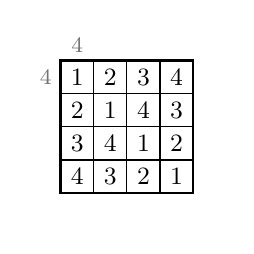
\begin{tikzpicture}[x=0.42cm,y=0.42cm]
\draw[line width=0.4pt] (1,0) -- (1,4);
\draw[line width=0.4pt] (0,1) -- (4,1);
\draw[line width=0.4pt] (2,0) -- (2,4);
\draw[line width=0.4pt] (0,2) -- (4,2);
\draw[line width=0.4pt] (3,0) -- (3,4);
\draw[line width=0.4pt] (0,3) -- (4,3);
\draw[line width=1pt] (0,0) rectangle (4,4);
\node at (0.5,3.5) {\small 1};
\node at (1.5,3.5) {\small 2};
\node at (2.5,3.5) {\small 3};
\node at (3.5,3.5) {\small 4};
\node at (0.5,2.5) {\small 2};
\node at (1.5,2.5) {\small 1};
\node at (2.5,2.5) {\small 4};
\node at (3.5,2.5) {\small 3};
\node at (0.5,1.5) {\small 3};
\node at (1.5,1.5) {\small 4};
\node at (2.5,1.5) {\small 1};
\node at (3.5,1.5) {\small 2};
\node at (0.5,0.5) {\small 4};
\node at (1.5,0.5) {\small 3};
\node at (2.5,0.5) {\small 2};
\node at (3.5,0.5) {\small 1};
\node[text=black!55] at (0.5,4.45) {\footnotesize 4};
\node[text=black!55] at (-0.45,3.5) {\footnotesize 4};
\path (-1,-1) rectangle (5,5);
\end{tikzpicture}}
\newcommand{\UfourSolb}{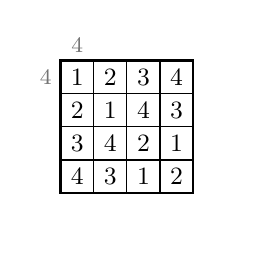
\begin{tikzpicture}[x=0.42cm,y=0.42cm]
\draw[line width=0.4pt] (1,0) -- (1,4);
\draw[line width=0.4pt] (0,1) -- (4,1);
\draw[line width=0.4pt] (2,0) -- (2,4);
\draw[line width=0.4pt] (0,2) -- (4,2);
\draw[line width=0.4pt] (3,0) -- (3,4);
\draw[line width=0.4pt] (0,3) -- (4,3);
\draw[line width=1pt] (0,0) rectangle (4,4);
\node at (0.5,3.5) {\small 1};
\node at (1.5,3.5) {\small 2};
\node at (2.5,3.5) {\small 3};
\node at (3.5,3.5) {\small 4};
\node at (0.5,2.5) {\small 2};
\node at (1.5,2.5) {\small 1};
\node at (2.5,2.5) {\small 4};
\node at (3.5,2.5) {\small 3};
\node at (0.5,1.5) {\small 3};
\node at (1.5,1.5) {\small 4};
\node at (2.5,1.5) {\small 2};
\node at (3.5,1.5) {\small 1};
\node at (0.5,0.5) {\small 4};
\node at (1.5,0.5) {\small 3};
\node at (2.5,0.5) {\small 1};
\node at (3.5,0.5) {\small 2};
\node[text=black!55] at (0.5,4.45) {\footnotesize 4};
\node[text=black!55] at (-0.45,3.5) {\footnotesize 4};
\path (-1,-1) rectangle (5,5);
\end{tikzpicture}}
\newcommand{\UfourSolc}{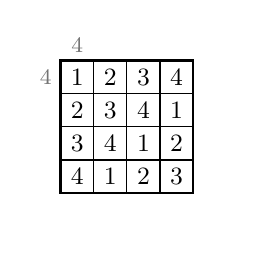
\begin{tikzpicture}[x=0.42cm,y=0.42cm]
\draw[line width=0.4pt] (1,0) -- (1,4);
\draw[line width=0.4pt] (0,1) -- (4,1);
\draw[line width=0.4pt] (2,0) -- (2,4);
\draw[line width=0.4pt] (0,2) -- (4,2);
\draw[line width=0.4pt] (3,0) -- (3,4);
\draw[line width=0.4pt] (0,3) -- (4,3);
\draw[line width=1pt] (0,0) rectangle (4,4);
\node at (0.5,3.5) {\small 1};
\node at (1.5,3.5) {\small 2};
\node at (2.5,3.5) {\small 3};
\node at (3.5,3.5) {\small 4};
\node at (0.5,2.5) {\small 2};
\node at (1.5,2.5) {\small 3};
\node at (2.5,2.5) {\small 4};
\node at (3.5,2.5) {\small 1};
\node at (0.5,1.5) {\small 3};
\node at (1.5,1.5) {\small 4};
\node at (2.5,1.5) {\small 1};
\node at (3.5,1.5) {\small 2};
\node at (0.5,0.5) {\small 4};
\node at (1.5,0.5) {\small 1};
\node at (2.5,0.5) {\small 2};
\node at (3.5,0.5) {\small 3};
\node[text=black!55] at (0.5,4.45) {\footnotesize 4};
\node[text=black!55] at (-0.45,3.5) {\footnotesize 4};
\path (-1,-1) rectangle (5,5);
\end{tikzpicture}}
\newcommand{\UfourSold}{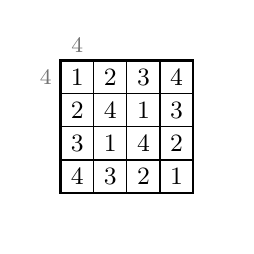
\begin{tikzpicture}[x=0.42cm,y=0.42cm]
\draw[line width=0.4pt] (1,0) -- (1,4);
\draw[line width=0.4pt] (0,1) -- (4,1);
\draw[line width=0.4pt] (2,0) -- (2,4);
\draw[line width=0.4pt] (0,2) -- (4,2);
\draw[line width=0.4pt] (3,0) -- (3,4);
\draw[line width=0.4pt] (0,3) -- (4,3);
\draw[line width=1pt] (0,0) rectangle (4,4);
\node at (0.5,3.5) {\small 1};
\node at (1.5,3.5) {\small 2};
\node at (2.5,3.5) {\small 3};
\node at (3.5,3.5) {\small 4};
\node at (0.5,2.5) {\small 2};
\node at (1.5,2.5) {\small 4};
\node at (2.5,2.5) {\small 1};
\node at (3.5,2.5) {\small 3};
\node at (0.5,1.5) {\small 3};
\node at (1.5,1.5) {\small 1};
\node at (2.5,1.5) {\small 4};
\node at (3.5,1.5) {\small 2};
\node at (0.5,0.5) {\small 4};
\node at (1.5,0.5) {\small 3};
\node at (2.5,0.5) {\small 2};
\node at (3.5,0.5) {\small 1};
\node[text=black!55] at (0.5,4.45) {\footnotesize 4};
\node[text=black!55] at (-0.45,3.5) {\footnotesize 4};
\path (-1,-1) rectangle (5,5);
\end{tikzpicture}}
\newcommand{\Msample}{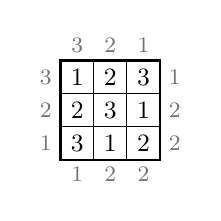
\begin{tikzpicture}[x=0.42cm,y=0.42cm]
\draw[line width=0.4pt] (1,0) -- (1,3);
\draw[line width=0.4pt] (0,1) -- (3,1);
\draw[line width=0.4pt] (2,0) -- (2,3);
\draw[line width=0.4pt] (0,2) -- (3,2);
\draw[line width=1pt] (0,0) rectangle (3,3);
\node at (0.5,2.5) {\small 1};
\node at (1.5,2.5) {\small 2};
\node at (2.5,2.5) {\small 3};
\node at (0.5,1.5) {\small 2};
\node at (1.5,1.5) {\small 3};
\node at (2.5,1.5) {\small 1};
\node at (0.5,0.5) {\small 3};
\node at (1.5,0.5) {\small 1};
\node at (2.5,0.5) {\small 2};
\node[text=black!55] at (0.5,3.45) {\footnotesize 3};
\node[text=black!55] at (0.5,-0.45) {\footnotesize 1};
\node[text=black!55] at (1.5,3.45) {\footnotesize 2};
\node[text=black!55] at (1.5,-0.45) {\footnotesize 2};
\node[text=black!55] at (2.5,3.45) {\footnotesize 1};
\node[text=black!55] at (2.5,-0.45) {\footnotesize 2};
\node[text=black!55] at (-0.45,2.5) {\footnotesize 3};
\node[text=black!55] at (3.45,2.5) {\footnotesize 1};
\node[text=black!55] at (-0.45,1.5) {\footnotesize 2};
\node[text=black!55] at (3.45,1.5) {\footnotesize 2};
\node[text=black!55] at (-0.45,0.5) {\footnotesize 1};
\node[text=black!55] at (3.45,0.5) {\footnotesize 2};
\path (-1,-1) rectangle (4,4);
\end{tikzpicture}}
\newcommand{\UsixSol}{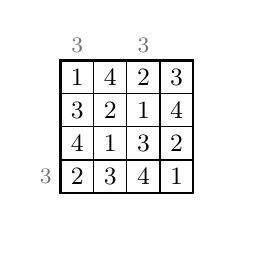
\begin{tikzpicture}[x=0.42cm,y=0.42cm]
\draw[line width=0.4pt] (1,0) -- (1,4);
\draw[line width=0.4pt] (0,1) -- (4,1);
\draw[line width=0.4pt] (2,0) -- (2,4);
\draw[line width=0.4pt] (0,2) -- (4,2);
\draw[line width=0.4pt] (3,0) -- (3,4);
\draw[line width=0.4pt] (0,3) -- (4,3);
\draw[line width=1pt] (0,0) rectangle (4,4);
\node at (0.5,3.5) {\small 1};
\node at (1.5,3.5) {\small 4};
\node at (2.5,3.5) {\small 2};
\node at (3.5,3.5) {\small 3};
\node at (0.5,2.5) {\small 3};
\node at (1.5,2.5) {\small 2};
\node at (2.5,2.5) {\small 1};
\node at (3.5,2.5) {\small 4};
\node at (0.5,1.5) {\small 4};
\node at (1.5,1.5) {\small 1};
\node at (2.5,1.5) {\small 3};
\node at (3.5,1.5) {\small 2};
\node at (0.5,0.5) {\small 2};
\node at (1.5,0.5) {\small 3};
\node at (2.5,0.5) {\small 4};
\node at (3.5,0.5) {\small 1};
\node[text=black!55] at (0.5,4.45) {\footnotesize 3};
\node[text=black!55] at (2.5,4.45) {\footnotesize 3};
\node[text=black!55] at (-0.45,0.5) {\footnotesize 3};
\path (-1,-1) rectangle (5,5);
\end{tikzpicture}}
\newcommand{\UnineA}{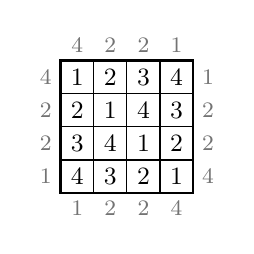
\begin{tikzpicture}[x=0.42cm,y=0.42cm]
\draw[line width=0.4pt] (1,0) -- (1,4);
\draw[line width=0.4pt] (0,1) -- (4,1);
\draw[line width=0.4pt] (2,0) -- (2,4);
\draw[line width=0.4pt] (0,2) -- (4,2);
\draw[line width=0.4pt] (3,0) -- (3,4);
\draw[line width=0.4pt] (0,3) -- (4,3);
\draw[line width=1pt] (0,0) rectangle (4,4);
\node at (0.5,3.5) {\small 1};
\node at (1.5,3.5) {\small 2};
\node at (2.5,3.5) {\small 3};
\node at (3.5,3.5) {\small 4};
\node at (0.5,2.5) {\small 2};
\node at (1.5,2.5) {\small 1};
\node at (2.5,2.5) {\small 4};
\node at (3.5,2.5) {\small 3};
\node at (0.5,1.5) {\small 3};
\node at (1.5,1.5) {\small 4};
\node at (2.5,1.5) {\small 1};
\node at (3.5,1.5) {\small 2};
\node at (0.5,0.5) {\small 4};
\node at (1.5,0.5) {\small 3};
\node at (2.5,0.5) {\small 2};
\node at (3.5,0.5) {\small 1};
\node[text=black!55] at (0.5,4.45) {\footnotesize 4};
\node[text=black!55] at (0.5,-0.45) {\footnotesize 1};
\node[text=black!55] at (1.5,4.45) {\footnotesize 2};
\node[text=black!55] at (1.5,-0.45) {\footnotesize 2};
\node[text=black!55] at (2.5,4.45) {\footnotesize 2};
\node[text=black!55] at (2.5,-0.45) {\footnotesize 2};
\node[text=black!55] at (3.5,4.45) {\footnotesize 1};
\node[text=black!55] at (3.5,-0.45) {\footnotesize 4};
\node[text=black!55] at (-0.45,3.5) {\footnotesize 4};
\node[text=black!55] at (4.45,3.5) {\footnotesize 1};
\node[text=black!55] at (-0.45,2.5) {\footnotesize 2};
\node[text=black!55] at (4.45,2.5) {\footnotesize 2};
\node[text=black!55] at (-0.45,1.5) {\footnotesize 2};
\node[text=black!55] at (4.45,1.5) {\footnotesize 2};
\node[text=black!55] at (-0.45,0.5) {\footnotesize 1};
\node[text=black!55] at (4.45,0.5) {\footnotesize 4};
\path (-1,-1) rectangle (5,5);
\end{tikzpicture}}
\newcommand{\UnineB}{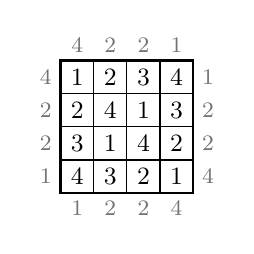
\begin{tikzpicture}[x=0.42cm,y=0.42cm]
\draw[line width=0.4pt] (1,0) -- (1,4);
\draw[line width=0.4pt] (0,1) -- (4,1);
\draw[line width=0.4pt] (2,0) -- (2,4);
\draw[line width=0.4pt] (0,2) -- (4,2);
\draw[line width=0.4pt] (3,0) -- (3,4);
\draw[line width=0.4pt] (0,3) -- (4,3);
\draw[line width=1pt] (0,0) rectangle (4,4);
\node at (0.5,3.5) {\small 1};
\node at (1.5,3.5) {\small 2};
\node at (2.5,3.5) {\small 3};
\node at (3.5,3.5) {\small 4};
\node at (0.5,2.5) {\small 2};
\node at (1.5,2.5) {\small 4};
\node at (2.5,2.5) {\small 1};
\node at (3.5,2.5) {\small 3};
\node at (0.5,1.5) {\small 3};
\node at (1.5,1.5) {\small 1};
\node at (2.5,1.5) {\small 4};
\node at (3.5,1.5) {\small 2};
\node at (0.5,0.5) {\small 4};
\node at (1.5,0.5) {\small 3};
\node at (2.5,0.5) {\small 2};
\node at (3.5,0.5) {\small 1};
\node[text=black!55] at (0.5,4.45) {\footnotesize 4};
\node[text=black!55] at (0.5,-0.45) {\footnotesize 1};
\node[text=black!55] at (1.5,4.45) {\footnotesize 2};
\node[text=black!55] at (1.5,-0.45) {\footnotesize 2};
\node[text=black!55] at (2.5,4.45) {\footnotesize 2};
\node[text=black!55] at (2.5,-0.45) {\footnotesize 2};
\node[text=black!55] at (3.5,4.45) {\footnotesize 1};
\node[text=black!55] at (3.5,-0.45) {\footnotesize 4};
\node[text=black!55] at (-0.45,3.5) {\footnotesize 4};
\node[text=black!55] at (4.45,3.5) {\footnotesize 1};
\node[text=black!55] at (-0.45,2.5) {\footnotesize 2};
\node[text=black!55] at (4.45,2.5) {\footnotesize 2};
\node[text=black!55] at (-0.45,1.5) {\footnotesize 2};
\node[text=black!55] at (4.45,1.5) {\footnotesize 2};
\node[text=black!55] at (-0.45,0.5) {\footnotesize 1};
\node[text=black!55] at (4.45,0.5) {\footnotesize 4};
\path (-1,-1) rectangle (5,5);
\end{tikzpicture}}
\newcommand{\Mtwelvea}{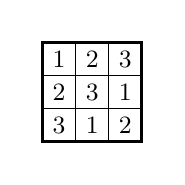
\begin{tikzpicture}[x=0.42cm,y=0.42cm]
\draw[line width=0.4pt] (1,0) -- (1,3);
\draw[line width=0.4pt] (0,1) -- (3,1);
\draw[line width=0.4pt] (2,0) -- (2,3);
\draw[line width=0.4pt] (0,2) -- (3,2);
\draw[line width=1pt] (0,0) rectangle (3,3);
\node at (0.5,2.5) {\small 1};
\node at (1.5,2.5) {\small 2};
\node at (2.5,2.5) {\small 3};
\node at (0.5,1.5) {\small 2};
\node at (1.5,1.5) {\small 3};
\node at (2.5,1.5) {\small 1};
\node at (0.5,0.5) {\small 3};
\node at (1.5,0.5) {\small 1};
\node at (2.5,0.5) {\small 2};
\path (-0.45,-0.45) rectangle (3.45,3.45);
\end{tikzpicture}\hspace{0.25cm}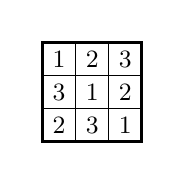
\begin{tikzpicture}[x=0.42cm,y=0.42cm]
\draw[line width=0.4pt] (1,0) -- (1,3);
\draw[line width=0.4pt] (0,1) -- (3,1);
\draw[line width=0.4pt] (2,0) -- (2,3);
\draw[line width=0.4pt] (0,2) -- (3,2);
\draw[line width=1pt] (0,0) rectangle (3,3);
\node at (0.5,2.5) {\small 1};
\node at (1.5,2.5) {\small 2};
\node at (2.5,2.5) {\small 3};
\node at (0.5,1.5) {\small 3};
\node at (1.5,1.5) {\small 1};
\node at (2.5,1.5) {\small 2};
\node at (0.5,0.5) {\small 2};
\node at (1.5,0.5) {\small 3};
\node at (2.5,0.5) {\small 1};
\path (-0.45,-0.45) rectangle (3.45,3.45);
\end{tikzpicture}\hspace{0.25cm}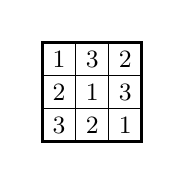
\begin{tikzpicture}[x=0.42cm,y=0.42cm]
\draw[line width=0.4pt] (1,0) -- (1,3);
\draw[line width=0.4pt] (0,1) -- (3,1);
\draw[line width=0.4pt] (2,0) -- (2,3);
\draw[line width=0.4pt] (0,2) -- (3,2);
\draw[line width=1pt] (0,0) rectangle (3,3);
\node at (0.5,2.5) {\small 1};
\node at (1.5,2.5) {\small 3};
\node at (2.5,2.5) {\small 2};
\node at (0.5,1.5) {\small 2};
\node at (1.5,1.5) {\small 1};
\node at (2.5,1.5) {\small 3};
\node at (0.5,0.5) {\small 3};
\node at (1.5,0.5) {\small 2};
\node at (2.5,0.5) {\small 1};
\path (-0.45,-0.45) rectangle (3.45,3.45);
\end{tikzpicture}\hspace{0.25cm}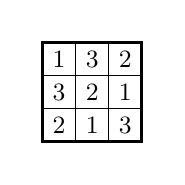
\begin{tikzpicture}[x=0.42cm,y=0.42cm]
\draw[line width=0.4pt] (1,0) -- (1,3);
\draw[line width=0.4pt] (0,1) -- (3,1);
\draw[line width=0.4pt] (2,0) -- (2,3);
\draw[line width=0.4pt] (0,2) -- (3,2);
\draw[line width=1pt] (0,0) rectangle (3,3);
\node at (0.5,2.5) {\small 1};
\node at (1.5,2.5) {\small 3};
\node at (2.5,2.5) {\small 2};
\node at (0.5,1.5) {\small 3};
\node at (1.5,1.5) {\small 2};
\node at (2.5,1.5) {\small 1};
\node at (0.5,0.5) {\small 2};
\node at (1.5,0.5) {\small 1};
\node at (2.5,0.5) {\small 3};
\path (-0.45,-0.45) rectangle (3.45,3.45);
\end{tikzpicture}\hspace{0.25cm}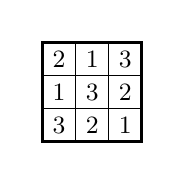
\begin{tikzpicture}[x=0.42cm,y=0.42cm]
\draw[line width=0.4pt] (1,0) -- (1,3);
\draw[line width=0.4pt] (0,1) -- (3,1);
\draw[line width=0.4pt] (2,0) -- (2,3);
\draw[line width=0.4pt] (0,2) -- (3,2);
\draw[line width=1pt] (0,0) rectangle (3,3);
\node at (0.5,2.5) {\small 2};
\node at (1.5,2.5) {\small 1};
\node at (2.5,2.5) {\small 3};
\node at (0.5,1.5) {\small 1};
\node at (1.5,1.5) {\small 3};
\node at (2.5,1.5) {\small 2};
\node at (0.5,0.5) {\small 3};
\node at (1.5,0.5) {\small 2};
\node at (2.5,0.5) {\small 1};
\path (-0.45,-0.45) rectangle (3.45,3.45);
\end{tikzpicture}\hspace{0.25cm}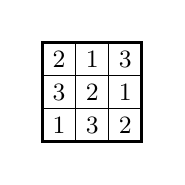
\begin{tikzpicture}[x=0.42cm,y=0.42cm]
\draw[line width=0.4pt] (1,0) -- (1,3);
\draw[line width=0.4pt] (0,1) -- (3,1);
\draw[line width=0.4pt] (2,0) -- (2,3);
\draw[line width=0.4pt] (0,2) -- (3,2);
\draw[line width=1pt] (0,0) rectangle (3,3);
\node at (0.5,2.5) {\small 2};
\node at (1.5,2.5) {\small 1};
\node at (2.5,2.5) {\small 3};
\node at (0.5,1.5) {\small 3};
\node at (1.5,1.5) {\small 2};
\node at (2.5,1.5) {\small 1};
\node at (0.5,0.5) {\small 1};
\node at (1.5,0.5) {\small 3};
\node at (2.5,0.5) {\small 2};
\path (-0.45,-0.45) rectangle (3.45,3.45);
\end{tikzpicture}}
\newcommand{\Mtwelveb}{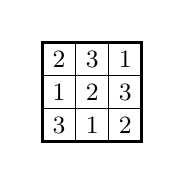
\begin{tikzpicture}[x=0.42cm,y=0.42cm]
\draw[line width=0.4pt] (1,0) -- (1,3);
\draw[line width=0.4pt] (0,1) -- (3,1);
\draw[line width=0.4pt] (2,0) -- (2,3);
\draw[line width=0.4pt] (0,2) -- (3,2);
\draw[line width=1pt] (0,0) rectangle (3,3);
\node at (0.5,2.5) {\small 2};
\node at (1.5,2.5) {\small 3};
\node at (2.5,2.5) {\small 1};
\node at (0.5,1.5) {\small 1};
\node at (1.5,1.5) {\small 2};
\node at (2.5,1.5) {\small 3};
\node at (0.5,0.5) {\small 3};
\node at (1.5,0.5) {\small 1};
\node at (2.5,0.5) {\small 2};
\path (-0.45,-0.45) rectangle (3.45,3.45);
\end{tikzpicture}\hspace{0.25cm}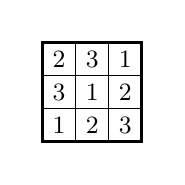
\begin{tikzpicture}[x=0.42cm,y=0.42cm]
\draw[line width=0.4pt] (1,0) -- (1,3);
\draw[line width=0.4pt] (0,1) -- (3,1);
\draw[line width=0.4pt] (2,0) -- (2,3);
\draw[line width=0.4pt] (0,2) -- (3,2);
\draw[line width=1pt] (0,0) rectangle (3,3);
\node at (0.5,2.5) {\small 2};
\node at (1.5,2.5) {\small 3};
\node at (2.5,2.5) {\small 1};
\node at (0.5,1.5) {\small 3};
\node at (1.5,1.5) {\small 1};
\node at (2.5,1.5) {\small 2};
\node at (0.5,0.5) {\small 1};
\node at (1.5,0.5) {\small 2};
\node at (2.5,0.5) {\small 3};
\path (-0.45,-0.45) rectangle (3.45,3.45);
\end{tikzpicture}\hspace{0.25cm}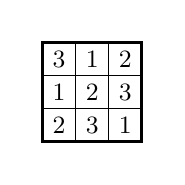
\begin{tikzpicture}[x=0.42cm,y=0.42cm]
\draw[line width=0.4pt] (1,0) -- (1,3);
\draw[line width=0.4pt] (0,1) -- (3,1);
\draw[line width=0.4pt] (2,0) -- (2,3);
\draw[line width=0.4pt] (0,2) -- (3,2);
\draw[line width=1pt] (0,0) rectangle (3,3);
\node at (0.5,2.5) {\small 3};
\node at (1.5,2.5) {\small 1};
\node at (2.5,2.5) {\small 2};
\node at (0.5,1.5) {\small 1};
\node at (1.5,1.5) {\small 2};
\node at (2.5,1.5) {\small 3};
\node at (0.5,0.5) {\small 2};
\node at (1.5,0.5) {\small 3};
\node at (2.5,0.5) {\small 1};
\path (-0.45,-0.45) rectangle (3.45,3.45);
\end{tikzpicture}\hspace{0.25cm}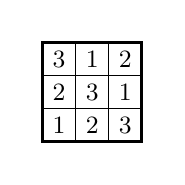
\begin{tikzpicture}[x=0.42cm,y=0.42cm]
\draw[line width=0.4pt] (1,0) -- (1,3);
\draw[line width=0.4pt] (0,1) -- (3,1);
\draw[line width=0.4pt] (2,0) -- (2,3);
\draw[line width=0.4pt] (0,2) -- (3,2);
\draw[line width=1pt] (0,0) rectangle (3,3);
\node at (0.5,2.5) {\small 3};
\node at (1.5,2.5) {\small 1};
\node at (2.5,2.5) {\small 2};
\node at (0.5,1.5) {\small 2};
\node at (1.5,1.5) {\small 3};
\node at (2.5,1.5) {\small 1};
\node at (0.5,0.5) {\small 1};
\node at (1.5,0.5) {\small 2};
\node at (2.5,0.5) {\small 3};
\path (-0.45,-0.45) rectangle (3.45,3.45);
\end{tikzpicture}\hspace{0.25cm}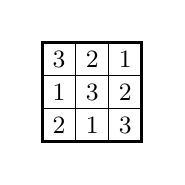
\begin{tikzpicture}[x=0.42cm,y=0.42cm]
\draw[line width=0.4pt] (1,0) -- (1,3);
\draw[line width=0.4pt] (0,1) -- (3,1);
\draw[line width=0.4pt] (2,0) -- (2,3);
\draw[line width=0.4pt] (0,2) -- (3,2);
\draw[line width=1pt] (0,0) rectangle (3,3);
\node at (0.5,2.5) {\small 3};
\node at (1.5,2.5) {\small 2};
\node at (2.5,2.5) {\small 1};
\node at (0.5,1.5) {\small 1};
\node at (1.5,1.5) {\small 3};
\node at (2.5,1.5) {\small 2};
\node at (0.5,0.5) {\small 2};
\node at (1.5,0.5) {\small 1};
\node at (2.5,0.5) {\small 3};
\path (-0.45,-0.45) rectangle (3.45,3.45);
\end{tikzpicture}\hspace{0.25cm}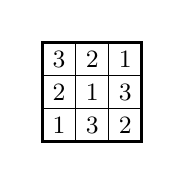
\begin{tikzpicture}[x=0.42cm,y=0.42cm]
\draw[line width=0.4pt] (1,0) -- (1,3);
\draw[line width=0.4pt] (0,1) -- (3,1);
\draw[line width=0.4pt] (2,0) -- (2,3);
\draw[line width=0.4pt] (0,2) -- (3,2);
\draw[line width=1pt] (0,0) rectangle (3,3);
\node at (0.5,2.5) {\small 3};
\node at (1.5,2.5) {\small 2};
\node at (2.5,2.5) {\small 1};
\node at (0.5,1.5) {\small 2};
\node at (1.5,1.5) {\small 1};
\node at (2.5,1.5) {\small 3};
\node at (0.5,0.5) {\small 1};
\node at (1.5,0.5) {\small 3};
\node at (2.5,0.5) {\small 2};
\path (-0.45,-0.45) rectangle (3.45,3.45);
\end{tikzpicture}}
